\chapter{Технологическая часть}
\setcounter{section}{2}
\section{Программная реализация инструментария \textit{Adaptor}}
\subsection{Выбор языка программирования}
\subsubsection{Рассмотрение альтернатив}
Ниже приведены возможные варианты выбора языка, разделённые по классам, и оценка их применимости в разработке системы.
\begin{itemize}
    \item Относительно низкоуровневые компилируемые языки (\textit{C}, \textit{C++}). Применимость этих языков в основном ограничена сложностью и низкой скоростью разработки на них в связи с недостаточно высоким уровнем абстрактности этих языков. Высокая производительность, которой можно достичь с помощью них, не является серьёзным преимуществом, поскольку реализация работающей системы на таких языках занимает значительно большее время, делая разговор о конечной производительности преждевременным.
    \item Более высокоуровневые компилируемые языки (\textit{Java}, \textit{C\#}). Эти языки работают на виртуальных машинах, что ограничивает их переносимость. В случае \textit{C\#}, полная современная реализация существует только для \textit{Windows}, что является неприемлемым в связи с тем, что конечная система должна работать и на \textit{Unix}--подобных операционных системах. Ещё одним недостатком можно назвать их компилируемость, поскольку это опять же снижает скорость разработки и значительно усложняет реализацию интерактивного окружения для проведения экспериментов.
    \item Современные императивные интерпретируемые языки (\textit{Ruby}, \textit{Python}). Эти языки позволяют вести разработку с высокой скоростью и хорошо приспособлены для разработки через тестирование (\textit{Test-Driven Development}, \cite{tdd}). Они хорошо переносимы и позволяют легко реализовать интерактивное окружение для работы с системой. Недостатком является относительно низкая скорость выполнения, что компенсируется более высокой скоростью разработки.
\end{itemize}

Другие семейства языков не рассматриваются ввиду низкой популярности. Это обусловлено тем, что язык реализации системы должен быть знаком большому количеству специалистов "--- так будет проще вести  разработку.


\subsubsection{Итоговое решение}
В качестве основного языка реализации системы был выбран \textit{Python}~\cite{python}. Это простой и удобный, популярный и хорошо поддерживаемый язык с большим количеством библиотек. Он более распространён \cite{langpop} и имеет большее количество библиотек, чем \textit{Ruby}. Он хорошо поддерживает современные методики разработки программ, такие, как \mbox{разработка через тестирование \cite{tdd}}, за счёт встроенных модулей для работы с автоматическими тестами.

В случае необходимости можно достигнуть высокой производительности с помощью интерпретатора \textit{PyPy}~\cite{pypy}. Для реализации сложной обработки данных можно использовать модуль \textit{scipy}~\cite{scipy} и для визуализации графиков "--- модуль \textit{matplotlib}~\cite{matplotlib}. Для реализации статистической обработки данных и машинного обучения можно воспользоваться одним из нескольких популярных модулей, среди которых \textit{Orange} \cite{orange} и \textit{sklearn} \cite{sklearn}.


\subsection{Репозиторий исходных кодов экспериментальных программ}
Инструментарий выполняет эксперименты по запуску программ, исходный код которых доступен экспериментатору. Экспериментатору должна быть доступна большая база исходных кодов для обеспечения возможности производить эксперименты над разнообразными программами, среди которых должны быть и похожие между собой. Последнее требование нужно ввиду необходимости обнаруживать похожесть программ в их поведении при изменении аппаратного обеспечения и настроек сборки.

В качестве репозитория предлагается использовать сервер распределённой системы контроля версий \cite{distributed-vcs}. Такая архитектура позволяет удобно работать с локальными копиями репозитория при необходимости произвести незначительные изменения для проверки какой-либо гипотезы относительно оптимизационного поведения программ. Она также позволяет отправлять локальные изменения на центральный сервер, что полезно для обмена исходными кодами между экспериментаторами. В отличие от централизованной системы контроля версий, распределённая система позволяет удалённым участникам разработки легко включиться в процесс развития системы (во многом за счёт более простого и мощного процесса ветвления версий кода). Кроме того, она позволяет использовать для размещения репозитория бесплатные службы вроде \textit{Github}~\cite{github} и \textit{Bitbucket}~\cite{bitbucket}, что устраняет необходимость в выделенном сервере системы контроля версий.


\subsubsection{Рассмотрение альтернатив}
Далее рассматриваются основные распределённые системы контроля версий с оценкой их применимости в разработке системы. Основным источником является веб-страница \cite{git-vs-hg}.
\begin{itemize}
    \item \textit{Mercurial}. Эта система контроля версий более проста в изучении и лучше поддерживает Windows. Вместе с тем, она в большей степени ограничивает разработчика "--- например, не позволяет переписывать историю изменений.
    \item \textit{Git}. Эта система версионирования является более мощной, чем \textit{Mercurial} и позволяет производить многие необходимые в процессе работы действия более быстро и удобно.
\end{itemize}


\subsubsection{Итоговое решение}
В связи с большой гибкостью и удобством для разработчика, в качестве репозитория исходных кодов был выбран \textit{Git}.

Стоит отметить, что на данный момент репозиторий исходных кодов тестовых программ является частью общего репозитория исходного кода описываемой системы. Этим также частично обусловлен выбор в пользу \textit{Git}, поскольку исторически исходный код инструментария находился в \textit{Git}. Также \textit{Git} более знаком автору.


\subsection{База данных экспериментов}
Для хранения данных об экспериментах необходима база данных. Традиционная реляционная база данных плохо подходит на эту роль, поскольку она требует наличия жёсткой схемы, которой следуют все таблицы, и все записи должны иметь одинаковый формат. Это представляет проблему в случае плохо определённой предметной области (такой, как наша исследовательская задача статистического анализа производительности программ), поскольку заранее неизвестно, какие свойства сущностей, сохраняемых в БД, являются важными, а какие --- нет. Это приводит к тому, что структура БД часто меняется по мере необходимости введения новых свойств, например, при добавлении в модель нового признака эксперимента по запуску программы.

Рассмотрим документо-ориентированные базы данных. Они позволяют хранить документы в каком-либо текстовом формате (обычно \textit{JSON}~\cite{json}) и не требуют одинаковой структуры всех документов. Поля документов могут добавляться и удаляться непосредственно по запросу пользователя. Это свойство особенно важно для нашей задачи. Также эти БД лучше масштабируются (т.\,е. лучше приспособлены к использованию в крупных распределённых системах).


\subsubsection{Рассмотрение альтернатив}
Далее приведен список документо-ориентированных БД с оценкой их применимости в нашей задаче. Основой для сравнения служит источник~\cite{nosql-comparison}.

\begin{itemize}
    \item \textit{MongoDB}. Это хранилище во многом похоже на реляционные БД. Оно использует свой бинарный протокол передачи данных и ориентировано на получение высокой производительности.
    \item \textit{CouchDB}. Это хранилище акцентировано на целостности хранимых данных и простоте в использовании. Оно поддерживает двустороннюю репликацию данных и представления данных через применение и свёртку (англ.~{map-reduce}~\cite{map-reduce}). Также имеется возможность построения приложения на \textit{JavaScript}, которое обеспечивает весь необходимый функционал БД (например, просмотр документов с определёнными свойствами). Хорошо подходит для ситуаций, когда данные накапливаются, но не изменяются.
    \item \textit{Redis}. Хранилище в памяти для быстро-изменяющихся данных с протоколом, похожем на \textit{Telnet}.
\end{itemize}

Другие альтернативы (\textit{HBase}, \textit{Cassandra}) не рассматриваются ввиду их специализации на экстремально больших объёмах данных (типичных для банков и поисковых машин) и не лучшей поддержки интерфейса к языку \textit{Python}.


\subsubsection{Итоговое решение}
В итоге в качестве БД была выбрана \textit{CouchDB}, поскольку она хорошо подходит для сильно распределённых систем (что важно для обеспечения работы отдельных исследователей в различных организациях) и накопления редко меняющихся данных. Поскольку в нашем случае эксперимент по оптимизации программы по определению не может быть изменён после проведения, это подходящий выбор.
Это хранилище также удобно в разработке "--- оно позволяет удобно организовать все функции для доступа к данным в виде отдельного приложения на диске "--- так называемого \textit{CouchApp}~\cite{couchapp}. Это позволяет хранить исходный код для работы с БД вместе с остальным исходным кодом инструментария.


\subsection{Установка инструментария \textit{Adaptor} на компьютер пользователя}
В рекомендуемом окружении "--- ОС \textit{Ubuntu 12.04} на платформе \textit{x86} или \textit{x86-64} "--- установка производится в полу-автоматическом режиме посредством использования системного пакетного менеджера \texttt{apt-get}.

Шаги, выполняемые в процессе установки в общем случае на любой платформе, приведены ниже. Шаги, отмеченные символом {*}, не являются необходимыми при выполнении установки в рекомендуемом окружении для проведения исследований.

\begin{enumerate}
    \item*\,Установить интерпретатор \textit{Python} версии не ниже 2.7.
    \item Установить \textit{CouchDB} версии не ниже 1.1.
    \item Установить \textit{CouchApp}.
    \item*\,Настроить переменные окружения и пути для использования установленных программ.
\end{enumerate}


\subsection{Расширяемость инструментария \textit{Adaptor}}
Инструментарий \textit{Adaptor} обеспечивает расширяемость в смысле возможности добавления новых модулей сборки, запуска и анализа данных.

Стоит отметить базовую поддержку сценариев исследований. Сценарий "--- это набор действий вида <<собрать программу>>, <<запустить программу с измерением времени>>, <<построить график зависимости времени от компилятора>> и т.\,д. Он может задаваться интерактивно или в исходном файле в виде функции языка программирования \textit{Python} с использованием \textit{API} инструментария в том же модуле, что и основной код системы, или в отдельном модуле (предпочтительно последнее). Система также предоставляет интерфейс для использования её в качестве модуля языка \textit{Python} сторонними пользователями. Полный набор доступных для использования в сценариях действий на данный момент описан только в исходном коде, однако это не является проблемой по следующим причинам. Во-первых, исходный код системы достаточно хорошо прокомментирован. Во-вторых, при использовании интерпретатора \textit{ipython} для работы с инструментарием, из комментариев и исходного кода генерируется минимальная документация.


\subsection{Платформа для использования инструментария \textit{Adaptor}}
Инструментарий \textit{Adaptor} протестирован в ОС~\textit{Linux} на \textit{x86}-совместимом процессоре ввиду распространённости данной аппаратной платформы, а также удобства разработки и ведения исследований под Linux.

Система использует функции, специфичные для ОС~\textit{Linux}, в ограниченном объёме. Для полнофункциональной работы инструментария необходимо портирование модуля сбора данных об аппаратном обеспечении. Все остальные модули системы независимы от ОС, на которой используется система, и должны также работать под \textit{Windows} или \textit{Mac}. Тестирование инструментария на этих ОС не производилось.


\subsection{Архитектура инструметария \textit{Adaptor}}
Инструментарий \textit{Adaptor} состоит из нескольких основных компонентов. Они перечислены ниже.

\begin{itemize}
    \item Компонент загрузки и установки основных переменных. Этот компонент осуществляет инициализацию инструментария и выполняет получение базового пути к каталогу системы, соединяется с базой данных и передаёт управление определённому сценарию исследования или пользователю.
    \item Компонент поддержания структуры рабочих путей. Этот компонент работает со стеком путей и позволяет пользователю переходить к под-каталогам инструментария различными способами:
    \begin{itemize}
        \item от корневого каталога, в котором расположен инструментарий;
        \item от корневого каталога, в котором расположен репозиторий исходных кодов исследуемых программ;
        \item по абсолютному пути в локальной операционной системе.
    \end{itemize}
    \item Компонент подготовки команд для сборки и запуска программ. Он осуществляет шаблонную подстановку заданных пользователем значений в заготовки команд.
    \item Компонент запуска подготовленных команд и обмена данными с запущенным процессом. Он осуществляет запуск в контролируемом окружении, измерение времени работы и приём-передачу потоков стандартного ввода, вывода и ошибок.
    \item Компонент калибровки измерения времени. Его описание можно найти ниже в подразделе с соответствующим названием.
    \item Компонент сравнения измеренного времени с заведомо известным. Осуществляет вычисление ошибки измерения.
    \item Компонент создания документов базы данных из полученных в рамках эксперимента сведений. Документы имеют формат JSON \cite{json} и создаются из внутренних структур данных инструментария для возможности последующего сохранения в базу данных.
\end{itemize}

Все компоненты реализованы в виде функций языка \textit{Python}. Применение объектной модели на данный момент не необходимо и перегружает код ненужными абстракциями.


\subsection{Эксперимент по оптимизации программы}
Эксперимент состоит в следующем.

\begin{enumerate}
	\item Система собирает программу с определёнными настройками сборки (см.~ниже).

	\item Система запускает программу в контролируемом окружении с определёнными настройками запуска и производит измерение интересующих метрик исполнения программы. Список метрик см.~ниже.

	На данный момент нас будет интересовать полное время исполнения.
	Список настроек исполнения см.~ниже.

	\item Система сохраняет данные о сборке и запуске программы в базу данных для последующего анализа и обработки.
\end{enumerate}

В случае компилятора \textit{gcc} настройки сборки включают в себя \cite{gcc-options}:
\begin{itemize}
    \item компилятор (команда для запуска);
    \item базовый уровень оптимизации (флаг \texttt{-O[n]}, где \texttt{n} "--- уровень оптимизации);
    \item набор флагов тонких настроек оптимизации (флаги семейства \texttt{-f[name]}, где \texttt{name} "--- имя определённого набора оптимизаций). Некоторые из этих флагов также имеют числовые параметры;
    \item путь к заголовочным файлам (опция \texttt{-I});
    \item путь к исходным файлам;
    \item параметры определения макросов (флаги вида \texttt{-D[MACRO]}, где \texttt{MACRO} "--- имя определяемого макроса);
    \item путь к исполняемому файлу, производимому компилятором.
\end{itemize}

Метрики исполнения могут быть следующими:
\begin{itemize}
    \item полное время исполнения программы;
    \item время исполнения программы по функциям;
    \item полный объём памяти, занимаемой программой и данными;
    \item объём памяти, занимаемой кодом программы;
\end{itemize}

\begin{samepage}
Настройки исполнения содержат:
\nopagebreak
\begin{itemize}
    \item путь к исполняемому файлу;
    \item источник ввода для стандартного потока ввода программы (перенаправление \texttt{stdin});
    \item потоки вывода для стандартного потока вывода и стандартного потока ошибок программы (перенаправление \texttt{stdout} и \texttt{stderr} соответственно);
    \item аргументы запуска, в т.ч. путь к обрабатываемому файлу данных (например, путь к файлу изображения для программы сжатия изображений).
\end{itemize}
\end{samepage}


\subsubsection{Время исполнения программы}
Точное измерение времени исполнения программы может представлять сложности ввиду возможных колебаний из-за изменения загрузки системы другими задачами. Принципиально, рекомендуется выполнять эксперименты на системе, не занятой другими задачами. Однако даже в таком случае системные процессы или разница в решениях, принятых планировщиком процессов, могут оказать значительное воздействие на измерение времени. Подробнее о механизмах, применяемых в планировщиках процессов в современных ОС и о возможном воздействии на время выполнения задачи, смотри источник~\cite{scheduling}.

Для устранения описанных проблем необходимо производить несколько запусков программы. Программа запускается 3 раза и берётся минимальное время её выполнения. Это время будет наиболее точно отражать производительность программно-аппаратной платформы, поскольку увеличение времени выполнения происходит в связи с интерференцией данного процесса с другими и общим состоянием системы. Как показали эксперименты (результаты в этой работе не приводятся), воздействие кэширования на производительность программы из тестового набора при многократном запуске при текущей реализации инструментария не наблюдается.

В случае внешнего измерения времени исполнения влияние оказывают также накладные расходы, связанные с запуском программы из системы. Для их исключения измерять время исполнения лучше изнутри программы и выводить его, например, в стандартный поток ошибок. Таким образом измерение времени производится в пакете тестирования производительности \textit{Polybench}~\cite{polybench}.

Внутреннее измерение времени исполнения обеспечивает большую точность, однако, оно требует поддержки на уровне исходного кода. Очевидно, что для универсального инструментария запуска оптимизационных экспериментов такое решение неприемлемо, поскольку должно быть возможно измерение времени выполнения программ, никак специально не подготовленных для этого.

По этой причине система измеряет время исполнения извне. Невысокая точность измерения при этом устраняется с помощью калибровки (см.~ниже). При этом также стоит отметить, что погрешность, вносимая внешним измерением, является систематической и не оказывает влияния на относительное время выполнения разных версий программы, что является наиболее важным в данной задаче.


\subsubsection{Калибровка времени исполнения программы}
\label{sssect:calibration}
Помимо отмеченных сложностей, есть сложность измерения маленьких интервалов времени. Если время исполнения программы находится на уровне 1 мс (таково временное разрешение системного вызова \textit{Unix} \texttt{gettimeofday}), то даже если запускать программу несколько раз, колебания измерений окажутся настолько большими, что сделают результат неточным. Для устранения этой проблемы предлагается специальный алгоритм калибровки, схема которого приведена ниже. Он также позволяет уменьшить влияние колебаний времени исполнения.

\begin{enumerate}
    \item Положить $n = 0, t = 0, d_{rel} = 1$.
    \item Исполнить программу однократно и измерить время её выполнения.
    \item Если время выполнения более 1 секунды, положить $n = -1$.
    \item Производить следующий цикл, пока $t < 1$ и $d_{rel} > 0,05$. Иначе перейти к шагу 9.
    \item Увеличить n на 1: $n = n + 1$.
    \item Вычислить число запусков программы как $number = 10^{n}$.
    \item Запустить программу $number$ раз, измеряя время выполнения. Повторить это 3 раза. Среди результатов выбрать минимум и присвоить его $t$. Вычислить относительную дисперсию результатов и присвоить её величине $d_{rel}$.
    \item Перейти к шагу 4.
    \item Получить время исполнения программы как $t / number$.
\end{enumerate}

В ряде случаев также используется сравнение измеренного времени исполнения с <<реальным>>. Хотя на практике сложно измерить время реального исполнения (т.е. за исключением времени запуска), время запуска можно вычислить, запустив программу, которая ничего не делает, и измерив время её исполнения. Затем можно вносить поправку на время запуска в каждое измерение (для устранения систематической методической погрешности). Проблема этого решения в том, что требуется очень точное измерение времени запуска пустой программы, но при применении тех же методов это принципиально невозможно --- время её исполнения также будет сильно колебаться в зависимости от загрузки системы и практически случайного воздействия планировщика задач в текущем состоянии системы.

Оценку предложенных методов измерения времени можно произвести путём сравнения измеренного времени исполнения с временем, заданным таймером с помощью вызова функции \texttt{usleep} стандартной библиотеки языка \textit{С} изнутри программы.

Стоит отметить, что существуют постоянные расходы на запуск программы из нашей системы и их можно вычесть из измеренного времени для повышения точности измерения. Для этого мы вычисляем время выполнения пустой программы, а затем вычитаем его из каждого измеренного результата выполнения реальных программ.


\subsubsection{Интерактивное окружение проведения экспериментов}
Для удобной работы с инструментарием рекомендуется использовать интерпретатор \textit{ipython}~\cite{ipython}. Он предоставляет графическую оболочку языка \textit{Python}, которая позволяет строить графики в том же окне, сохранять сессии использования интерпретатора и имеет хорошую поддержку автодополнения команд и документации. На рисунке~\ref{img:besselj} приведён снимок экрана этой графической оболочки с встроенным графиком.

\begin{figure}[tbp]
    \center{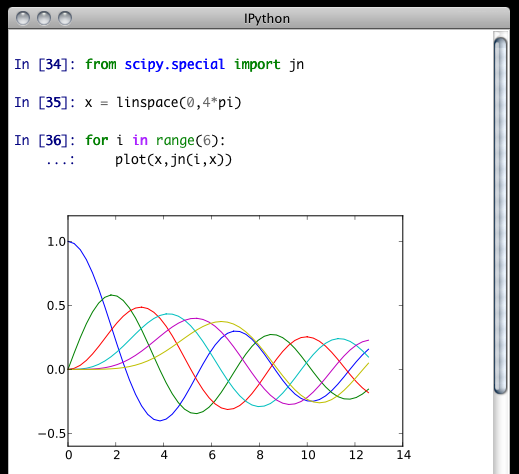
\includegraphics[width=0.6\linewidth]{besselj}}
    \caption{Cнимок экрана графической оболочки \textit{ipython} с встроенным графиком}
    \label{img:besselj}
\end{figure}

\subsection{Конвейер обработки данных в системе Orange}
\label{orange-pipeline}

На рисунке \ref{img:series30} изображён конвейер статистической обработки данных в системе \textit{Orange}. Здесь он приведён целиком, в уменьшенном виде, для понимания общего расположения компонентов.

Конвейер имеет такой вид для всех трёх серий экспериментов. Далее мы рассмотрим части конвейера по отдельности и опишем каждый компонент, используемый в схеме анализа данных, изображённой на указанном выше рисунке.

\begin{figure}[tbp]
    \center{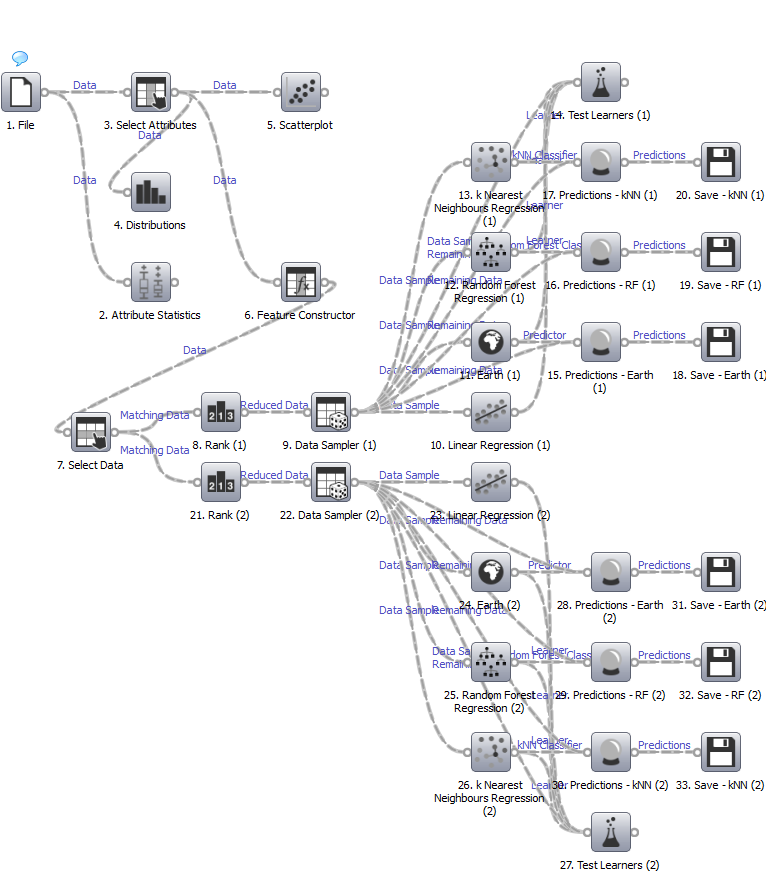
\includegraphics[scale=0.375]{series30}}
    \caption{Конвейер обработки данных в системе \textit{Orange}}
    \label{img:series30}
\end{figure}

Первая часть конвейера "--- предварительная обработка данных перед построением модели. Она изображена на рисунке~\ref{img:series30-1}.

\begin{figure}[tbp]
    \center{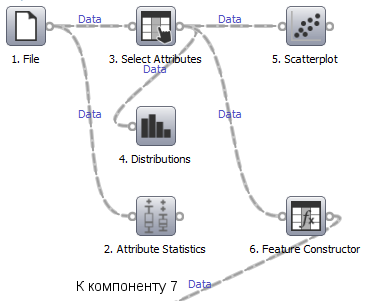
\includegraphics[scale=1]{series30-1}}
    \caption{Конвейер обработки данных в системе \textit{Orange}. Часть 1 "--- предварительная обработка}
    \label{img:series30-1}
\end{figure}

Обработка данных в системе начинается с чтения входных данных в формате \textit{CSV} из файла "--- за это отвечает компонент \texttt{1.\,File}, находящийся в левом верхнем углу схемы. Отчёт по этому компоненту представлен на рисунке \ref{img:1-File}. Опишем формат входного файла.

\begin{figure}[tbp]
    \center{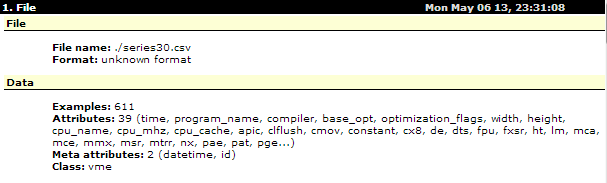
\includegraphics[scale=0.75]{1-File}}
    \caption{Компонент \texttt{1.\,File}. Входные данные в файле \textit{CSV}}
    \label{img:1-File}
\end{figure}

Входной файл содержит таблицу, в которой столбцы "--- это названия свойств эксперимента, полученных во время его выполнения в инструментарии, а строки "--- собственно значения этих свойств. Приведём отрывок файла для пояснения его структуры (рисунок \ref{img:series.csv}). Многоточия означают опущенные части файла "--- поскольку число свойств достигает сорока, представить файл полностью не представляется возможным ввиду ограниченной ширины страницы. Свойство \texttt{id} также представлено в сокращённом виде "--- символы \texttt{..} означают опущенные части строки.

\Rotatebox{90}{
    \begin{minipage}{1.25\linewidth}
        \begin{figure}[H]
            \fontsize{10}{12}
            \begin{verbatim}
            id datetime time program_name compiler base_opt width height cpu_name cpu_mhz cpu_cache ...
            51..16 2013-04-17 22:25:29 0.0041661978 symm gcc None 64 64 Intel(R) Xeon(R) ... 2666.76 6144 ...
            51..6d 2013-04-17 22:25:14 1.3440570831 symm gcc None 256 256 Intel(R) Xeon(R) ... 2666.76 6144 ...
            51..0b 2013-04-17 22:24:57 0.121064496 symm gcc None 128 128 Intel(R) Xeon(R) ... 2666.76 6144 ...
            \end{verbatim}
            \caption{Отрывок входного файла}
            \label{img:series.csv}
        \end{figure}
    \end{minipage}
}
\clearpage

Итак, первая строка файла "--- названия свойств. \texttt{id} "--- уникальный идентификатор эксперимента, \texttt{datetime} "--- время его проведения в GMT, \texttt{time} "--- время исполнения программы, \texttt{program_name} "--- название программы, \texttt{compiler} "--- название используемого компилятора, \texttt{base_opt} "--- базовый уровень оптимизации программы компилятором, \texttt{optimization_flags} "--- дополнительные настройки оптимизации, \texttt{width} "--- число столбцов в обрабатываемой матрице, \texttt{height} "--- число строк в обрабатываемой матрице, \texttt{cpu_name} "--- название процессора, на котором исполнялась программа, \texttt{cpu_mhz} "--- частота процессора, \texttt{cpu_cache} "--- объём кэша третьего уровня. Все остальные свойства, начиная с \texttt{apic} и заканчивая \texttt{vme} "--- двоичные свойства наличия у процессора поддержки определённой возможности, такой как, например, набора инструкций \textit{SSE}.

Отметим, что пунктирные линии на схеме обозначают передачу данных из одного компонента обработки данных в другой. Схема представляет собой дерево с корнем в узле \texttt{1.\,File}, причём данные передаются от корня к листьям. Таким образом, из узлов, которые не имеют дочерних, информация дальше не передаётся. Если у узла несколько дочерних узлов, данные передаются от родителя каждому ребёнку данного узла.

Компонент \texttt{2.\,Attribute~Statistics} используется для сбора и показа статистических показателей различных признаков экспериментов, содержащихся в наборе данных -- например, таких, как среднее и медианное значение признака. Выводимые им изображения можно найти в Приложении.

Компонент \texttt{3.\,Select~Attributes} (рисунок \ref{img:3-Select-Attributes}) применяется с целью установления структуры набора данных "--- в нём определяется, какие свойства экспериментов являются исходными данными для моделирования (признаками), а какие "--- выходными данными (предсказанными значениями). В данном случае все свойства экспериментов, кроме свойства \texttt{time} (время исполнения программы), являются признаками. Свойство \texttt{time} предсказывается моделью.

\begin{figure}[tbp]
    \center{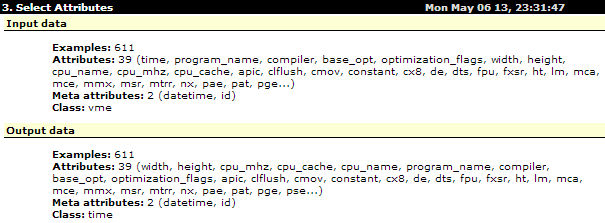
\includegraphics[scale=0.75]{3-Select-Attributes}}
    \caption{Компонент \texttt{3.\,Select~Attributes}. Определение структуры входных данных}
    \label{img:3-Select-Attributes}
\end{figure}

Компонент \texttt{4.\,Distributions} отображает распределения различных атрибутов набора данных. Эти графики можно найти в Приложении.

Компонент \texttt{5.\,Scatterplot} строит точечные графики зависимости времени исполнения программы от других свойств эксперимента. Пример такого графика можно найти в Приложении. На нём завершается предварительный анализ входных данных.

Компонент \texttt{6.\,Feature Constructor} используется для создания дополнительного свойства эксперимента из уже присутствующих в наборе данных "--- свойства \texttt{size}, определяемого как $size = height \cdot width$ и имеющего смысл агрегированного размера обрабатываемой программой \texttt{symm} матрицы.

Компонент \texttt{7.\,Select~Data} (рисунок \ref{img:7-Select-Data}) может использоваться для фильтрации данных по различным признакам. Например, он может быть использован для удаления из набора данных всех экспериментов, для которых измеренное время исполнения оказалось менее 0,001 с вследствие артефактов измерения. Такая фильтрация может увеличить качество предсказания, поскольку результаты, которые очевидно являются шумом, удаляются из набора данных. Однако, в конечных версиях рассмотренных моделей данный компонент не был задействован, поскольку он требует тонкой настройки и снижает степень автоматизации моделирования.

\begin{figure}[tbp]
    \center{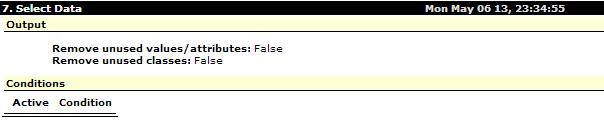
\includegraphics[scale=0.75]{7-Select-Data}}
    \caption{Компонент \texttt{7.\,Select~Data}. Выбор данных из набора}
    \label{img:7-Select-Data}
\end{figure}

На этом предварительная обработка данных завершается и начинается собственно построение модели. Компоненты под номерами с 8 по 20 и с 20 по 33 полностью аналогичны. Они представляют собой две ветви конвейера, в одной из которых (с компонентами 8--20) используется простейшая модель на основе единственного признака, а в другой (с компонентами 20--33) "--- более сложная модель на основе четырёх или пяти признаков.

Опишем обе ветви конвейера, начиная с части, отвечающей за ранжирование признаков и выборку объектов. Эта часть схемы изображена на рисунке~\ref{img:series30-2}.

\begin{figure}[tbp]
    \center{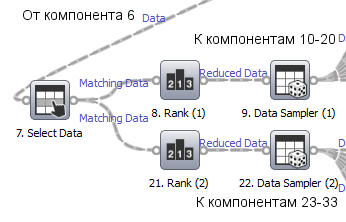
\includegraphics[scale=1]{series30-2}}
    \caption{Конвейер обработки данных в системе \textit{Orange}. Часть 2 "--- ранжирование признаков и выборка объектов}
    \label{img:series30-2}
\end{figure}

Компонент \texttt{8.\,Rank~(1)} (рисунок \ref{img:8-Rank-1}) и его аналог \texttt{21.\,Rank~(2)}  выбирает $S$ наиболее значимых признаков набора данных, при этом $S = 1$ для компонента 8 и $S = 4$ или $S = 5$ для компонента 21. Выбор $S = 4$ или $S = 5$ зависит от результата работы алгоритма выделения важных признаков и для первой серии экспериментов $S = 4$, а для второй и третьей "--- $S = 5$. Согласно рассуждениям, приведённым ниже в разделе~\ref{choice-of-feature-ranking-algorithm}, в качестве алгоритма ранжирования признаков во всех случаях используется алгоритм \textit{Earth}.

\begin{figure}[tbp]
    \center{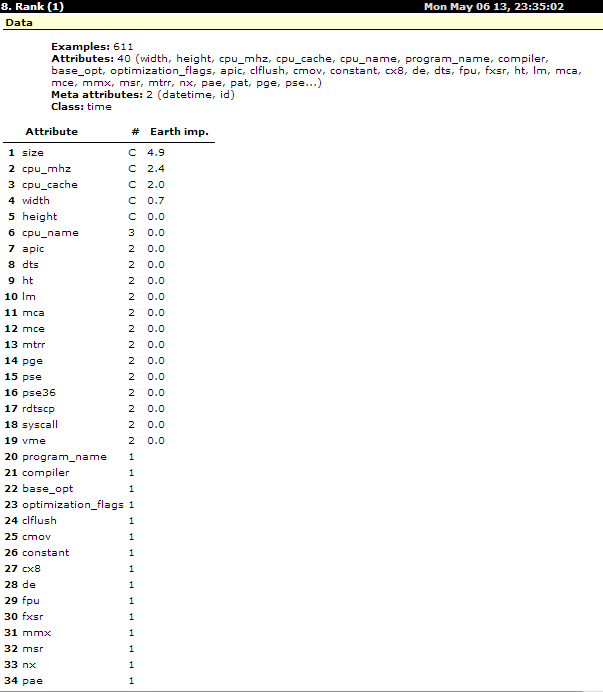
\includegraphics[scale=0.75]{8-Rank-1}}
    \caption{Компонент \texttt{8.\,Rank~(1)}. Выбор признаков}
    \label{img:8-Rank-1}
\end{figure}

Остановимся подробнее на выборе алгоритма ранжирования признаков.

\paragraph{Алгоритм ранжирования признаков}
\label{choice-of-feature-ranking-algorithm}

В системе статистической обработки данных Orange доступны следующие алгоритмы ранжирования признаков модели: \textit{Relief~F, MSE, Earth Importance} и \textit{Random Forest Importance}. В ходе изучения третьей серии экспериментов были получены результаты ранжирования признаков, показанные на рисунке~\ref{img:ranking-full}.

\begin{figure}[tbp]
    \center{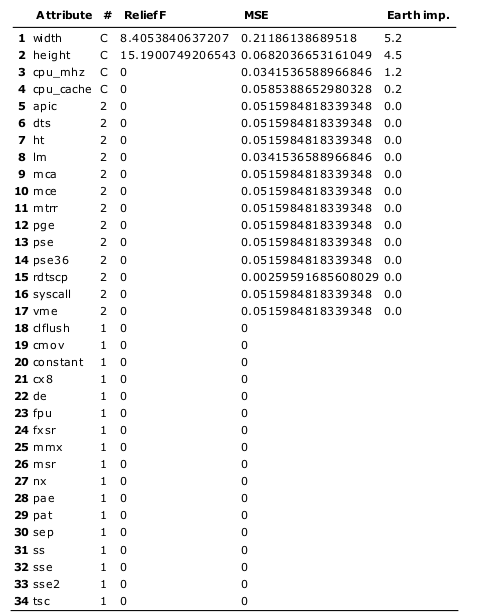
\includegraphics[scale=0.75]{ranking-full}}
    \caption{Сравнение алгоритмов ранжирования признаков модели}
    \label{img:ranking-full}
\end{figure}

Как можно видеть, алгоритм \textit{Relief~F} показал результаты, целиком отбрасывающие влияние свойств \texttt{cpu_mhz} и \texttt{cpu_cache}, а также всех остальных особенностей аппаратной платформы. Это заведомо неверно, поскольку известно, что характеристики аппаратного обеспечения влияют на производительность программы. Этот алгоритм выделил только два самых очевидных свойства, оказывающих влияние на производительность.

Алгоритм \textit{MSE} также присвоил наибольшие веса свойствам \texttt{width} и \texttt{height}, а на третье место по важности поставил \texttt{cpu_cache}, что выглядит разумно. Однако, данный алгоритм присвоил одинаковые веса многим признакам, которые просто коррелируют с изменением свойств \texttt{cpu_mhz} и \texttt{cpu_cache}, но не обнаружил корреляции -- таким образом, свойства \texttt{apic, dts} и другие получили вес $0,05159...$. При этом истинно важный признак \texttt{cpu_mhz} был оценён важностью, меньшей чем у всех этих коррелирующих признаков, что свидетельствует о невозможности применения этого алгоритма для нашей задачи.

Алгоритм \textit{Earth Importance} выявил все четыре признака, которые являются важными в нашей модели -- число строк и столбцов в обрабатываемой матрице, частоту используемого процессора и объём его кэша. При этом <<паразитные>> коррелирующие признаки не были оценены алгоритмом как важные "--- таким образом мы избавляемся от лишних свойств в модели и делаем её минимально необходимой для адекватного описания предметной области.

Алгоритм \textit{Random Forest Importance} отработал на нашем наборе данных некорректно, вызвав программную ошибку в системе Orange. Он был исключён из дальнейшего рассмотрения.

Таким образом, мы выбираем \textit{Earth Importance} в качестве алгоритма ранжирования признаков.

Теперь продолжим рассмотрение конвейера обработки данных в системе \textit{Orange}.

Компоненты \texttt{9.\,Data~Sampler~(1)} и \texttt{22.\,Data~Sampler~(2)} производят случайный отбор 70\% данных из набора в учебный набор, а остальных 30\% "--- в проверочный набор данных. Это необходимо для проведения перекрёстной проверки, которая в данном случае является одно-проходной ввиду ограниченных ресурсов времени и невысокой степени автоматизации осуществления перекрёстной проверки в системе \textit{Orange}. При этом компонент 9 работает с моделью, построенной на основе единственного признака, который был оценён, как наиболее важный, компонентом 8. Компонент 22 работает с моделью на основе четырёх или пяти признаков, наиболее важных по результатам работы компонента 21. Далее мы не будем останавливаться на различиях моделей в ветвях (8--20) и (20--33).

\begin{figure}[tbp]
    \center{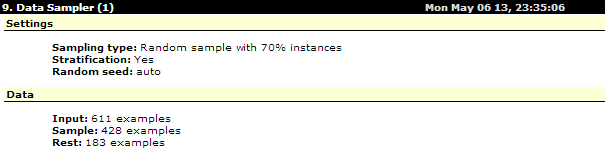
\includegraphics[scale=0.75]{9-Data-Sampler-1}}
    \caption{Компонент \texttt{9.\,Data~Sampler~(1)}. Отбор объектов в обучающую и проверочную выборки}
    \label{img:9-Data-Sampler-1}
\end{figure}

На этом вторая часть схемы заканчивается и мы переходим собственно к обучению предсказателей для двух моделей "--- простейшей (с одним признаком) и более сложной (с четырьмя или пятью признаками).

На рисунках~\ref{img:series30-3}~и~\ref{img:series30-4} представлены две последние части конвейера обработки данных в \textit{Orange}. Они полностью аналогичны и отличаются тем, что первая (описывающая компоненты~10--20) получает данные от компонента~9, а вторая (компоненты~23--33) "--- от компонента~22. Это данные, включающие в себя один признак эксперимента и несколько (четыре или пять) признаков эксперимента, соответственно.

\begin{figure}[tbp]
    \center{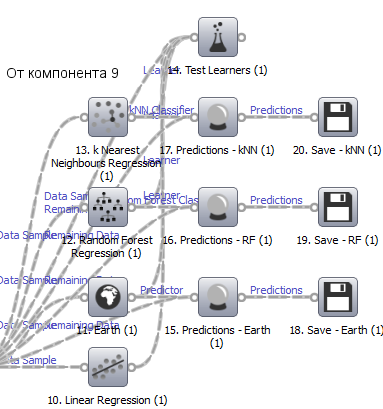
\includegraphics[scale=1]{series30-3}}
    \caption{Конвейер обработки данных в системе \textit{Orange}. Часть 3 "--- построение простейшей модели}
    \label{img:series30-3}
\end{figure}

Компоненты \texttt{10.\,Linear~Regression~(1)} и \texttt{23.\,Linear~Regression~(2)} строят модели линейной регрессии на основе экспериментальных данных. Эти модели являются образцовыми. Это значит, что качество результатов данных моделей является нижней границей для качества результатов любых других моделей. Поскольку линейная регрессия является простейшим предсказателем, рассмотрение моделей, которые дают результаты хуже, чем линейная регрессия, не имеет смысла. Модели из компонентов 10 и 23 передаются в компоненты 14 и 27 соответственно, где те сравниваются с другими предсказателями по нескольким метрикам (см. ниже).

\begin{figure}[tbp]
    \center{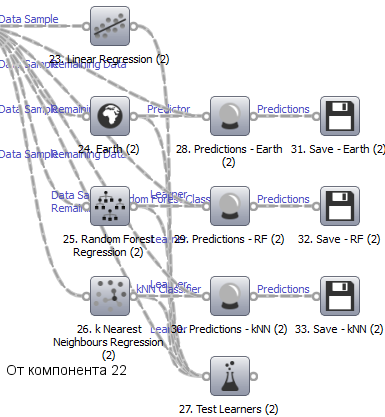
\includegraphics[scale=1]{series30-4}}
    \caption{Конвейер обработки данных в системе \textit{Orange}. Часть 4 "--- построение более сложной модели}
    \label{img:series30-4}
\end{figure}

Компоненты \texttt{11.\,Earth~(1), 12.\,Random~Forest Regression~(1), 13.\,k~Nearest~Neighbours Regression~(1)} и \texttt{24.\,Earth~(2), 25.~Random~Forest Regression~(2), 26.\,k~Nearest~Neighbours Regression~(2)} являются модулями построения предсказателей \textit{Earth, Random~Forest} и \textit{kNN} для ветвей (8--20) и (20--33) соответственно.

\begin{figure}[tbp]
    \center{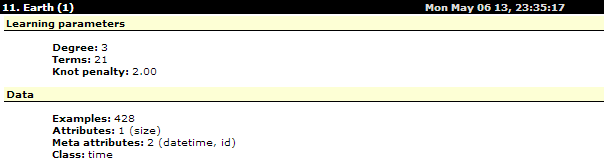
\includegraphics[scale=0.75]{11-Earth-1}}
    \caption{Компонент \texttt{11.\,Earth~(1)}. Предсказатель \textit{Earth} для модели с одним признаком}
    \label{img:11-Earth-1}
\end{figure}

\begin{figure}[tbp]
    \center{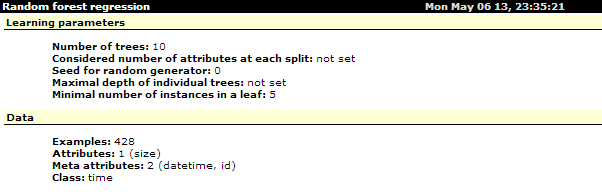
\includegraphics[scale=0.75]{12-RF-1}}
    \caption{Компонент \texttt{12.\,Random~Forest~(1)}. Предсказатель \textit{Random~Forest} для модели с одним признаком}
    \label{img:12-RF-1}
\end{figure}

\begin{figure}[tbp]
    \center{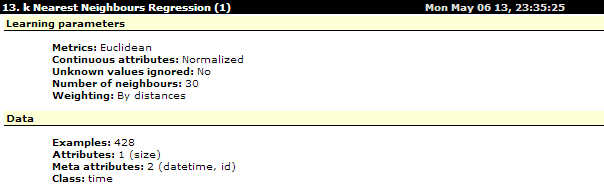
\includegraphics[scale=0.75]{13-kNN-1}}
    \caption{Компонент \texttt{13.\,kNN~(1)}. Предсказатель \textit{k~Nearest~Neighbours} для модели с одним признаком}
    \label{img:13-kNN-1}
\end{figure}

\begin{figure}[tbp]
    \center{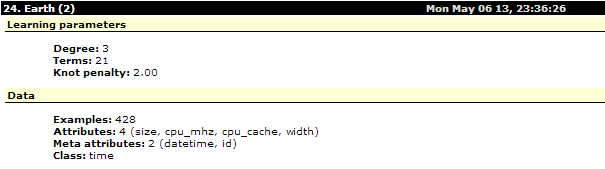
\includegraphics[scale=0.75]{24-Earth-2}}
    \caption{Компонент \texttt{24.\,Earth~(2)}. Предсказатель \textit{Earth} для модели с четырьмя признаками}
    \label{img:24-Earth-2}
\end{figure}

\begin{figure}[tbp]
    \center{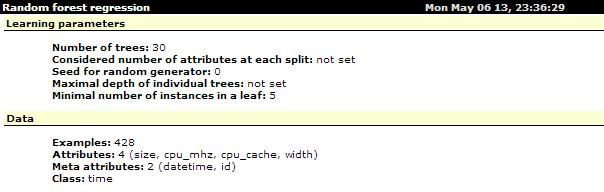
\includegraphics[scale=0.75]{25-RF-2}}
    \caption{Компонент \texttt{25.\,Random~Forest~(2)}. Предсказатель \textit{Random~Forest} для модели с четырьмя признаками}
    \label{img:25-RF-2}
\end{figure}

\begin{figure}[tbp]
    \center{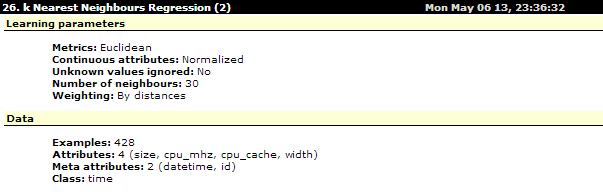
\includegraphics[scale=0.75]{26-kNN-2}}
    \caption{Компонент \texttt{26.\,kNN~(2)}. Предсказатель \textit{k~Nearest~Neighbours} для модели с четырьмя признаками}
    \label{img:26-kNN-2}
\end{figure}

После обучения предсказателей их параметры передаются в компоненты сравнения качества результатов \texttt{14.\,Test~Learners~(1)} и \texttt{27.\,Test~Learners~(2)}. Кроме этого, они используются для построения предсказаний в компонентах \texttt{15.\,Predictions - Earth~(1), 16.\,Predictions - RF~(1), 17.\,Predictions - kNN~(1)} и {28.\,Predictions - Earth~(2), 29.\,Predictions - RF~(2), 30.\,Predictions - kNN~(2)} соответсвенно.

\begin{figure}[tbp]
    \center{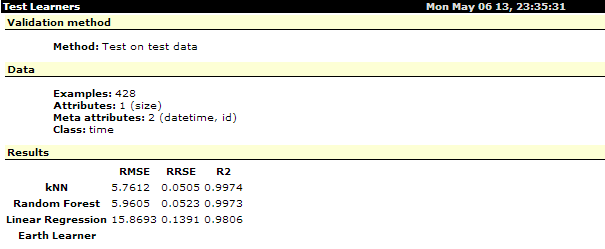
\includegraphics[scale=0.75]{14-Test-Learners-1}}
    \caption{Компонент \texttt{26.\,Test~Learners~(2)}. Сравнение предсказателей для модели с одним признаком}
    \label{img:14-Test-Learners-1}
\end{figure}

\begin{figure}[tbp]
    \center{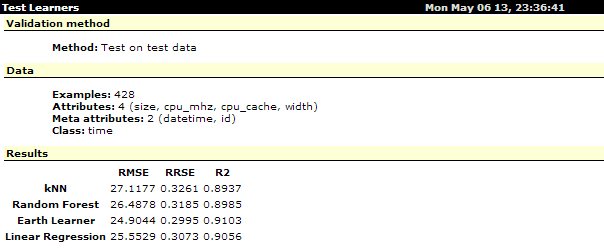
\includegraphics[scale=0.75]{27-Test-Learners-2}}
    \caption{Компонент \texttt{27.\,Test~Learners~(2)}. Сравнение предсказателей для модели с четырьмя признаками}
    \label{img:27-Test-Learners-2}
\end{figure}

После построения предсказаний, они сохраняются в файлах \textit{CSV} с помощью компонентов \texttt{18.\,Save - Earth~(1), 19.\,Save - RF~(1), 20.\,Save - kNN~(1)} и \texttt{31.\,Save - Earth~(2), 32.\,Save - RF~(2), 33.\,Save - kNN~(2)} в формате, аналогичном формату исходного файла, загруженного компонентом \texttt{1.\,File}.


\subsection{Выводы}
В рамках конструкторской части дипломного проекта была построена комплексная система, состоящей из набора модулей, разработанных на языке программирования \textit{Python}, и схемы статистической обработки данных в программе \textit{Orange}.